\chapter{7 TeV and 8 TeV Differential Cross Section Measurement}
\label{c:Differential_Cross_Section}

\section{Introduction}
\label{s:xsections_introduction}
This analysis measures the normalised differential \ttbar cross section in the semi-leptonic channel and is
carried out on 2011 and 2012 data recorded from the CMS detector. The measurement is carried out with respect
to the following global variables is carried out:
\begin {itemize}
  \item {\met, the missing transverse energy in an event}
  \item {\HT, the sum of the jet transverse momenta in an event}
  \item {\st, the sum of the observed transverse momenta in an event}
  \item {\mt, the transverse mass of the leptonically decaying W boson}
  \item {\wpt, the transverse momentum of the leptonically decaying W boson}
\end{itemize}

Previous analyses using 7~TeV data investigating \met and using 8~TeV data investigatin all the global
variables listed above can be found in \cite{CMS-PAS-TOP-12-019} and \cite{CMS-PAS-TOP-12-042} respectively.

This investigation is motivated primarily by the importance of understanding \ttbar events since they are a
significant background in many new physics analyses. It is also helpful in understanding QCD and event
generators. Rare Standard Model processes such as $\ttbar + W\rightarrow l\nu$ or $\ttbar + Z\rightarrow
\nu\bar{\nu}$ would appear in \met distribution tail, and $\ttbar + X$ where $X$ is massive would appear in
the \HT and \st distributions. There are also possible new physics scenarios such as stop pair production,
$\tilde{t}\bar{\tilde{t}} \rightarrow t\tilde{\chi_0} \bar{t}\bar{\tilde{\chi_0}}$ which could show
hints of dark matter.

\section{Data and Simulated Samples}
\label{s:data_and_simulated_samples}

\subsection{Data}
\label{ss:data}

Data collected in 2011 at a centre-of-mass energy of 7~TeV and in 2012 at a centre-of-mass energy of 8~TeV are
used. The datasets are determined by the triggers that were used to record them. For 7~TeV, the ElectronHad
dataset is used in the electron channel. It was recorded with triggers that select based on a single, isolated
electron and additional jets. At 8~TeV, the SingleElectron dataset was used for the electron channel which is
based on a single, isolated electron. In the muon channel, the SingleMu dataset was used for both
centre-of-mass energies, requiring a single, isolated muon. See Section~\ref{s:event_selection} for more
details about triggers. The datasets used are shown in Tables~\ref{tab:datasets7TeV} and {tab:datasets8TeV} in
Appendix~\ref{a:datasets}. Only data that is certified as “golden”, which is defined as data taken with the
detector working without any major faults, used. The masks used to filter out data taken in other periods are
specified in Table~\ref{tab:JSONfiles} in Appendix~\ref{a:datasets}.

\subsection{Simulated Samples}
\label{ss:simulated_samples}
The Monte Carlo generators used in this analysis are MadGraph \cite{madgraph}, PYTHIA \cite{pythia8}, POWHEG
\cite{powheg_Nason,powheg_Frixione,powheg_Alioli}, HERWIG \cite{herwig} and MC$@$NLO
\cite{mcatnlo_Frixione1, mcatnlo_Frixione2}.

The signal for this analysis is the production of a \ttbar pair which decays semi-leptonically, \ie each of
the t quarks decays to a W boson and a b jet, with one of the W bosons decaying hadronically to two jets and
the other decaying leptonically to a lepton (electron or muon) and an associated neutrino.

Additional, lower energy jets, can be produced from other scatterings in the same proton-proton interaction
and from gluon radiation from quarks in the decay. Events with W bosons or Z bosons and additional jets are a
significant background to semi-leptonic \ttbar analyses. In the case of W + jets, leptonically decaying W
bosons and additional jets would provide a similar event signature to that of a semi-leptonic \ttbar decay.
However, in general, these processes can be removed from the signal selection because the final decay products
in W + jets events have lower energies than those from semi-leptonic \ttbar decays, since the top quark has a
high mass. Another characteristic of W + jets events is that the jets are less likely to be the necessary b
jets in \ttbar events. Similarly, Z + jets events can mimic \ttbar events where the leptonic decay of Z
bosons to a lepton and an anti-lepton. In these cases, a veto on a second lepton together with jet
multiplicity requirements removes much of this background, although misidentification and misreconstruction
of leptons as jets could still mean some of these events still pass the signal selection, although this
contamination would be small. TODO:FEYNMANN DIAGRAM OF W & Z PRODUCTION.
%TODO: FEYNMANN DIAGRAM OF W & Z + JETS EVENTS

The QCD events that can form a background to \ttbar analyses, with the multi-jet final states resulting from
gluon-gluon fusion and quark-antiquark annihilation from proton proton collisions. At high orders, sufficient
numbers of jets can be produced to produce an event signature similar to that of \ttbar events. The leptons
required for this to happen can come from jets that are misreconstructed and misidentified as leptons, or from
the b and c quark decays. In the muon channel, it is possible to use isolation requirements to identify and
remove a jet of high enough energy that it leaves signals in the muon chambers, because it will also deposit
much energy in the calorimeters. Fake leptons caused by misreconstruction and misidentification, although not
a regular occurrence, form a significant background because the QCD cross section is large at the centre of
mass energies in this analysis. Fake leptons contained in b and c jets will not begin from the primary vertex
and so can be mostly excluded from the signal selection using their distinct track signature compared to prompt
leptons.

On the other hand, the electron channel poses a more problematic QCD background, due mainly to the conversion
of photons, whether produced at the interaction point or through subsequent decays and radiation, into
electrons and positrons. The identification and removal of such events has been described in
Section~\ref{ss:electron_reconstruction}. However, the large uncertainty in the cross section of QCD events,
large contamination from higher order processes with additional jets in the signal region of this analysis and
the difficulty in Monte Carlo modelling of such contributions lead to significant disagreements in the numbers
of events passing the signal selection in data and in simulation. Therefore, the QCD background is
modelled using a data driven method, decribed in Section~\ref{ss:qcd_selection}.

Table~\ref{monte_carlo_samples} shows the Monte Carlo signal and background samples used in this analysis. Top
pair production is modelled using MadGraph, single top events are modelled with POWHEG, W and Z boson plus
jets production is modelled using MadGraph and QCD multi-jet events are modelled with PYTHIA. In all cases,
PYTHIA is used to model radiation and hadronisation processes.





A simultaneous fit is done with three templates in bins of each variable.
The binning choice is made based on two variables: purity (equation) and stability (equation). The purity of a
bin is sensitive to events moving into/out of a bin and the stability is sensitive to events moving inout/out
of a bin. The bins for each global variable are selected such that each bin has purity and stability values of
0.5 or greater, meaning that at least half of the events created in a bin remain in that bin.
	
Electrons can be faked by jets, so the electron scale factors could be different in ttbar events than in
events from which the scale factors were derived because our events contain a lot more activity than events
from which the scale factors were derived.
For muons it is not so bad because muons leave a much cleaner signal inside CMS and there is no risk of jets
faking muons.
	
We use the lepton trigger, identification and isolation scale factors provided by the Muon POG for both 7 TeV
and 8 TeV. However, for electrons, although we have 8 TeV scale factors provided by the EGamma POG, we have
had to derive scale factors ourselves for 7 TeV because not provided (and the trigger we use is not included
in the 7 TeV Summer 11 Legacy datasets).
The hadronic leg of the electronHad trigger needs to be measured in relation to the 4 jets. ASK ABOUT THIS
	 
Remember:
- V\_Jets template combined over all global variable bins.
- QCD template also inclusive over all global variable bins
	
Within the framework of this analysis, prompt leptons are considered as those which come
from W or Z boson or from tau-lepton decays. These leptons are usually well isolated, whereas
misidentified leptons originate either from semi-leptonic heavy flavor decays within jets or are
simply misreconstructed genuine jets. In both cases these leptons are generally not isolated.

Tau energy: The met energy systematics are electron energy up/down, muon energy up/down and tau energy
up/down. These systematics (and JES) are applied to both monte carlo and data. We found that the tau energy is
susprisingly high, considerably higher than the electron and muon energy systematics. We may select taus in
our signal region unintentionally although we don't select on taus. The signature of ttbar events with taus
can mimic the signature of electron + jets or muon + jets ttbar events. The image shows how taus decay. The W
from a top could decay to a tau, which would then decay either to a tau neutrino and a virtual W which then
decays to two jets which would be very close together (and therefore reconstructed as a single jet). Or, the
virtual W could decay to a lepton (electron or muon) and an associated neutrino). These signatures could fake
our signal, and therefore end up in our ttbar signal. In our unfolding, we remove fakes. However, we use the
shape of the fakes in the central to subtract from the signal distribution in the tau energy up/down
variations. The effect is not so pronounced in the electron up/down and muon up/down variations because there
are not many electrons or muons in the fakes. Luke found that \~14\% of the TTJet events we select on are NOT
from the decay we are looking for. This was by dividing the number of events in the fake ST distribution in
the unfolding histogram file by the number of events in the measured distribution (i.e. signal) in the same
file. The electron channel was actually ~13.5\% and the muon channel was actually ~13.9\%. The shape
comparison between the fakes and the signal shows that there are more fakes in the higher MET bins, which is
why the error in those bins is larger. These are likely to come from semi-leptonic tau events (where the tau
decays to a lepton and a neutrino); tau tau, e tau or mu tau where the tau decays hadronically; or ee, emu or mumu events where one of the leptons is lost (probably low fraction as well). So most of our fakes will include at least one tau. Since semi-leptonic tau would need to
decay leptonically, these taus are not identified and, I assume, not included in the MET uncertainty.

Looking at the shape difference between the central and tau up/down MET distributions, there is a significant
different (though not by much). Since this affects data, the difference goes through the fit, and the
unfolding, and is what we see in the final result. The difference in normalisation in the most affected bin is
\~6\%, suggesting that we have more than 6\% tau contamination overall (not sure if that is a correct
assumption). The normalisation across the bins does not change, of course, i.e. the sum of events in the bins
of, in this case MET, remain the same in the central measurement and in the tau energy up/down variations.
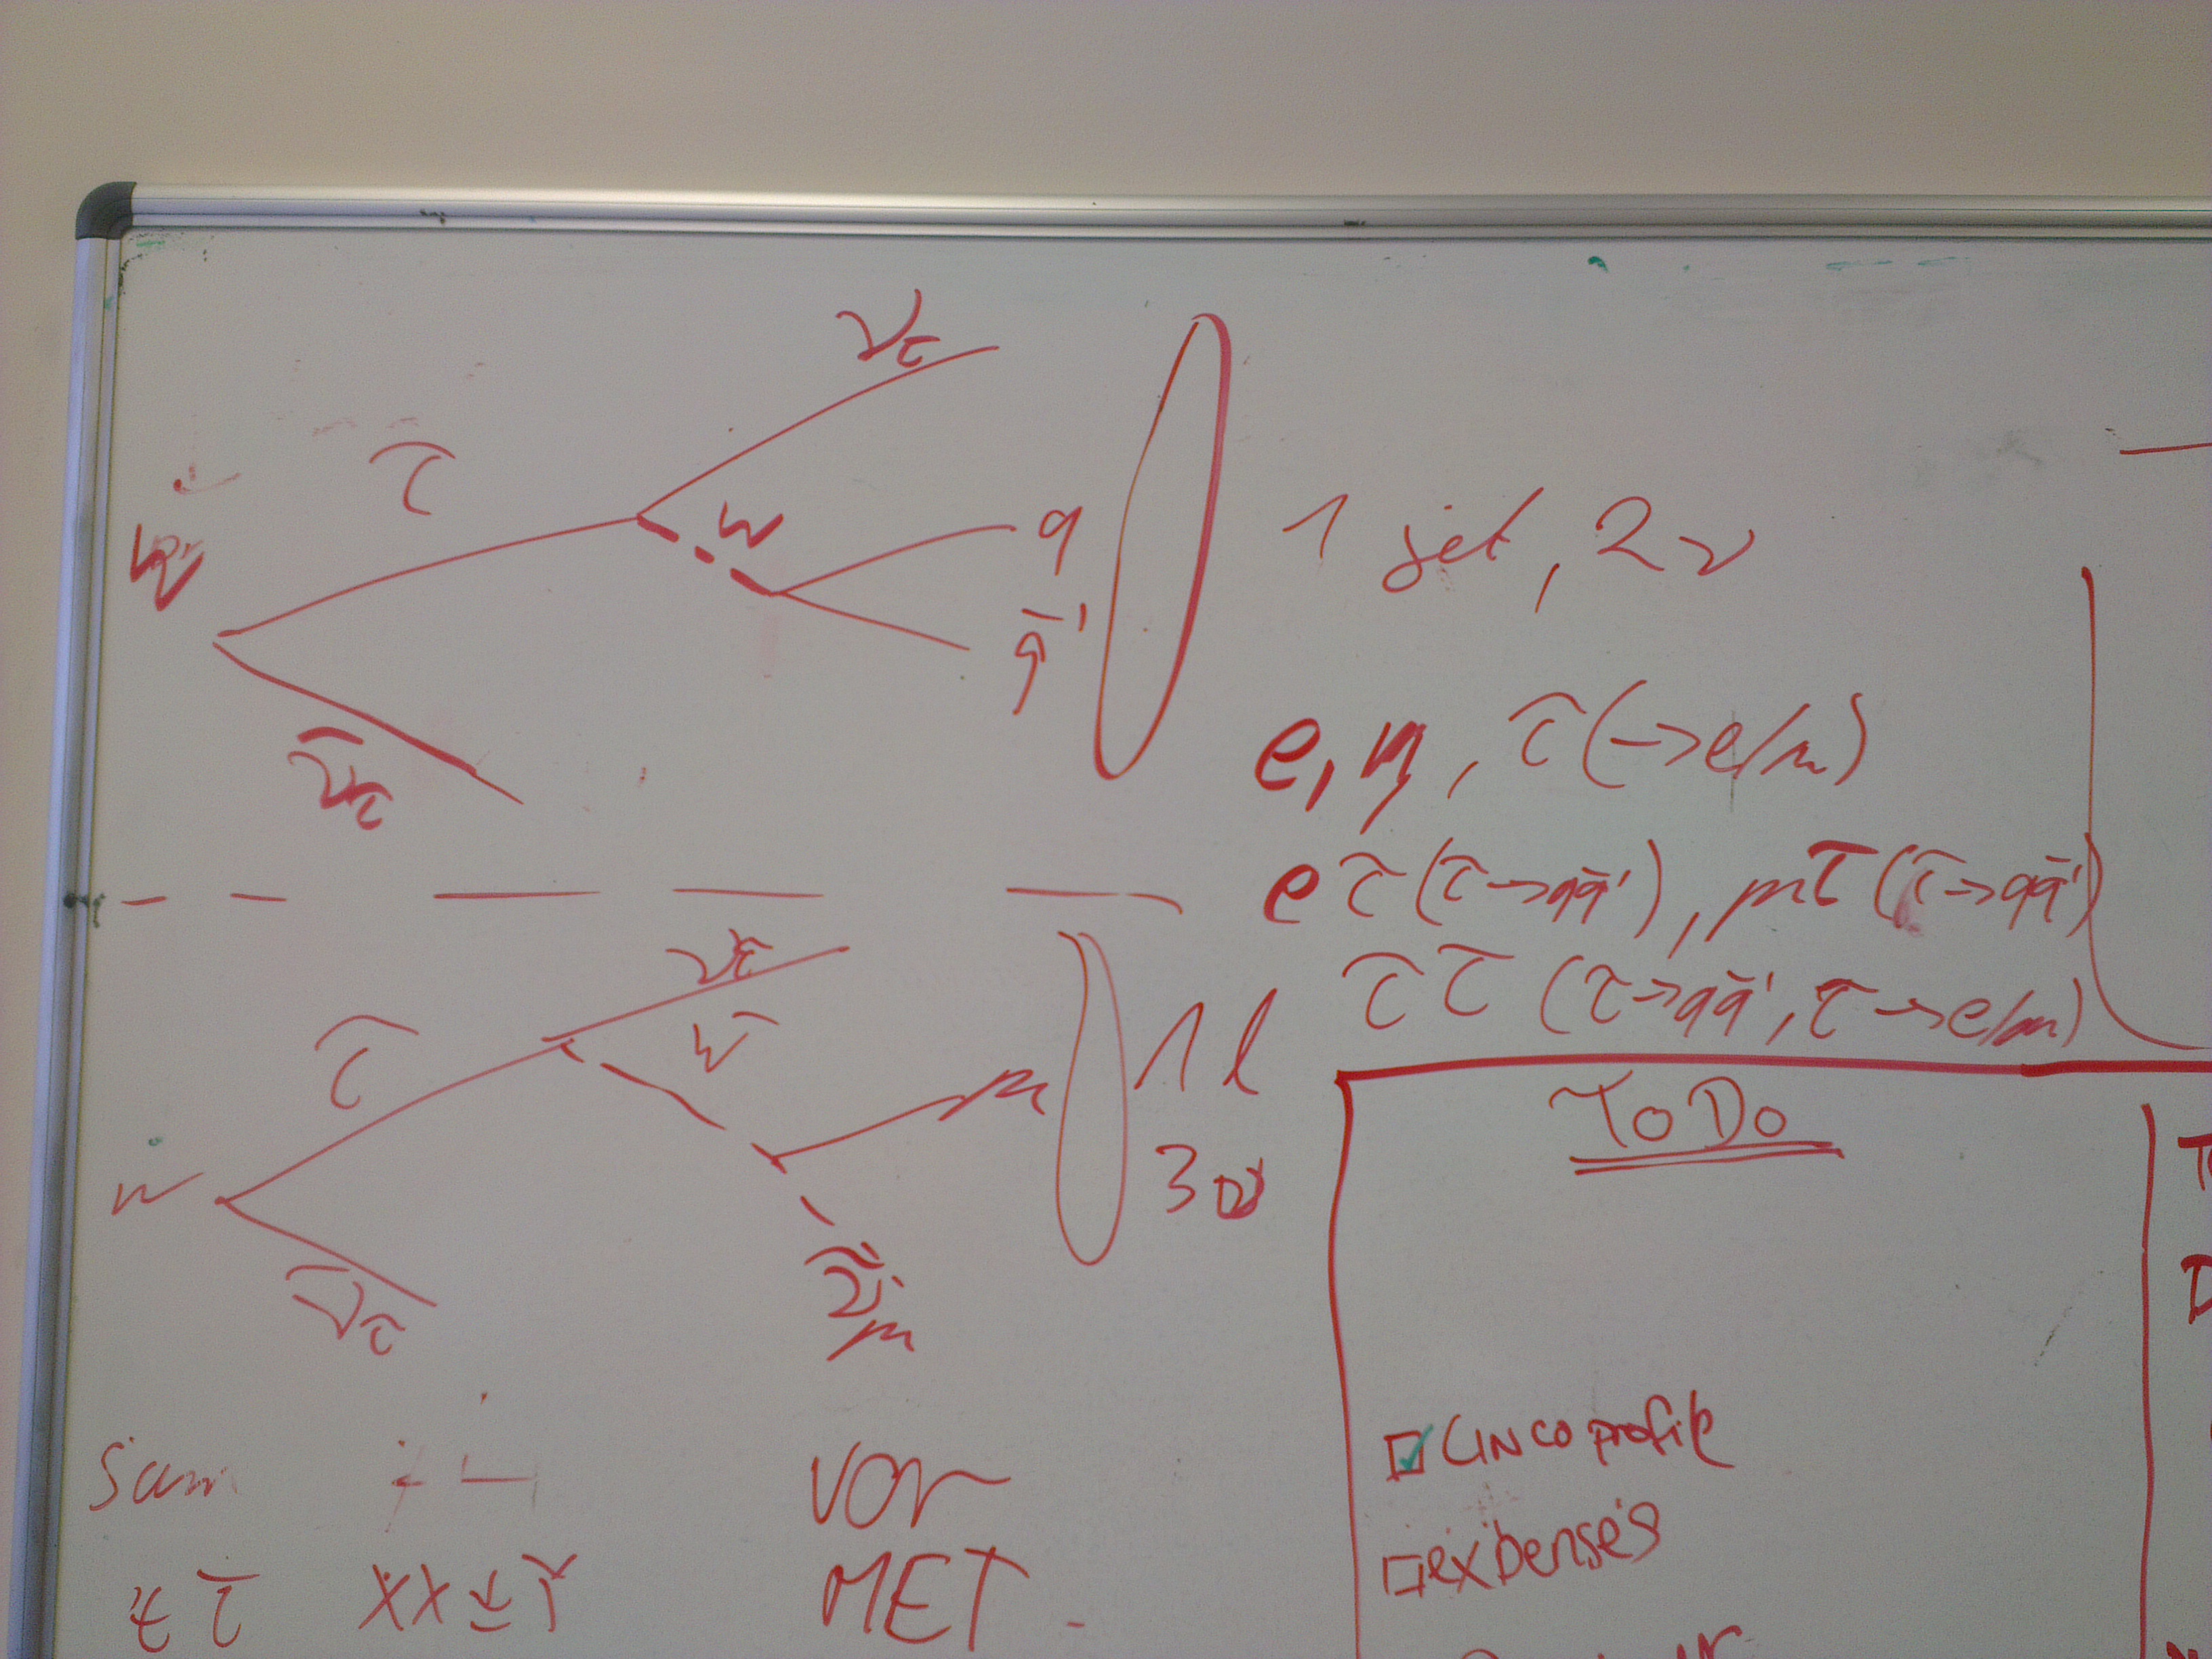
\includegraphics[width=\textwidth]{Chapters/04_Analysis/04b_XSections/Images/IMG_20150219_160840.jpg}

\section{Event Selection}
\label{s:event_selection}

\subsection{Data}
\label{ss:data_selection}

\subsection{QCD}
\label{ss:qcd_selection}
